\documentclass[12pt]{{memoir}}
\usepackage{graphicx}
\usepackage[overlay]{textpos}
\usepackage[hidelinks,pdfusetitle]{hyperref}
\usepackage{xfrac}
\usepackage[paperwidth=7.5in,paperheight=10.0in,top=.5in,bottom=.5in,left=.25in,right=.25in]{geometry}

\newcommand\Hline{%
\hline\raisebox{0pt}[1.125em]{}}
\newcommand\dupfootnote[1]{%
\textsuperscript{\ref{#1}}}
\newcommand\sepfootnote{%
\textsuperscript{,\,}}

\interfootnotelinepenalty=10000
\begin{document}
\title{Retro 6k Bundled Application User's Guide}
\author{Maggie\,David P.\,K. Haynes}
\pagestyle{empty}
\begin{center}
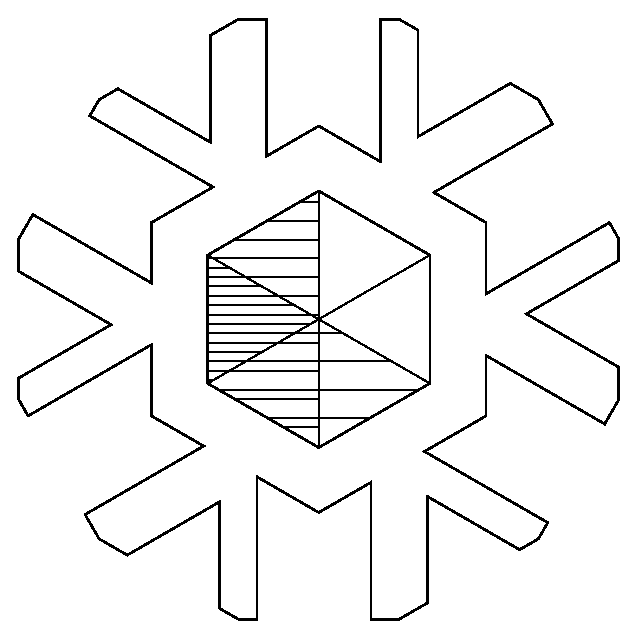
\includegraphics{../common-src/logolineart}

\vspace{\stretch{.25}}
{\sffamily\bfseries\Huge{}Retro 6k\\Fantasy Computer\\Entertainment System

\vspace{\stretch{1}}
Bundled Application User's Guide\par}
\vspace*{\stretch{1}}
{\sffamily\bfseries\large\theauthor\par}
\end{center}
\vspace*{\stretch{3}}
\cleartoverso
\vspace*{\stretch{2}}
\begin{center}
\noindent{}Haiku can be fun\\
but they don't always make sense.\\
Refrigerator.\par
\end{center}

\vspace*{\stretch{3}}
\cleartorecto
\tableofcontents*
\clearpage
\pagestyle{headings}

\vspace*{3in}
\section*{Conventions Used In This Document}

Nothing established yet.

\chapter{Marquee}

This program was my sister Erica's idea. The idea is simple: take some text the user has entered, enlarge it, and scroll it across the screen. Of course, I had to add some neat little features along the way.

\section{Text Entry Mode}

Marquee starts in text-entry mode. Text entry works as most computer users would expect. The text being edited here is a message up to 127 characters long, which will be displayed in marquee mode. Although the message is displayed across up to four lines on the screen in text-entry mode, semantically there are no line breaks. Don't worry if a word starts at the end of a line on the screen and continues on the next line; it's still in one piece as far as the computer is concerned. Any graphic character from the Retro 6k Stock Character Set\footnote{See Retro 6k Programmer's Guide} except for the right half solid block, card suits, astrological symbols, and quadruple cross. Those are interpreted as special keystrokes and/or not loaded into memory in Marquee.

Text-entry mode can be accessed by pressing \textsf{Shift+Enter} or \textsf{Ctrl+Shift+}\texttt{M} in any other mode\footnote{\label{marquee:f:nye}Not yet implemented.}. Pressing \textsf{Enter} or \textsf{Ctrl+}\texttt{M} in marquee mode also activates text-entry mode.

Changes made to the message in text-entry mode are effective immediately, and will remain when the user leaves text-entry mode by any means.

\section{Text Formatting Mode}

In text-formatting mode, the user can adjust the horizontal and vertical scale, slant, weight\dupfootnote{marquee:f:nye}, and interletter spacing\dupfootnote{marquee:f:nye} of the text in the marquee. Additionally, the speed at which the text scrolls across the screen may be adjusted. Simultaneously, a preview of the current settings is shown on the right half of the screen\dupfootnote{marquee:f:nye}. Changing the horizontal scale affects the range of allowed weight settings. Changing the weight setting affects the range of allowed spacing settings. Pressing \textsf{Esc} or \textsf{Shift+F1} reverts the settings to the values they had when text-formatting mode was activated.

Text-formatting mode can be accessed by pressing \textsf{Ctrl+}\texttt{K} or \textsf{Shift+F11} in any other mode.

\section{Color Painting Mode}

In color-painting mode, the user can change the foreground and background colors for each of 36 rows of the screen.\dupfootnote{marquee:f:nye} 32 different colors are available at a time.

Color-painting mode can be accessed by pressing \textsf{Ctrl+}\texttt{C} or \textsf{Shift+F3} in any other mode.\dupfootnote{marquee:f:nye}

\subsection{Palette Editing Mode}

In palette-editing mode, the user can change the 32 colors that are available for color-painting mode.\dupfootnote{marquee:f:nye}\sepfootnote\footnote{There are 256 possible colors that can be produced. This is a hardware limitation of the Retro 6k Fantasy Computer Entertainment System.}

Palette-editing mode can be accessed by pressing \textsf{Ctrl+}\texttt{P} or \textsf{Shift+}\texttt{0} in color-painting mode.\dupfootnote{marquee:f:nye}

\section{Marquee Mode}

In marquee mode, the text entered by the user scrolls across the screen in a large size. While marquee mode is active, the cartridge may be removed, and the marquee will continue to scroll.\dupfootnote{marquee:f:nye} However, leaving marquee mode without the 6k Marquee cartridge inserted will likely crash the Retro 6k Fantasy Computer Entertainment System.

Marquee mode can be accessed by pressing \textsf{Enter} or \textsf{Ctrl+}\texttt{M} in any other mode.

\cleartoverso
\pagestyle{empty}
\vspace*{\stretch{1}}

\noindent\thetitle\hfill\textcopyright2019--20 \theauthor

\end{document}
